\documentclass[twoside]{book}

% Packages required by doxygen
\usepackage{fixltx2e}
\usepackage{calc}
\usepackage{doxygen}
\usepackage[export]{adjustbox} % also loads graphicx
\usepackage{graphicx}
\usepackage[utf8]{inputenc}
\usepackage{makeidx}
\usepackage{multicol}
\usepackage{multirow}
\PassOptionsToPackage{warn}{textcomp}
\usepackage{textcomp}
\usepackage[nointegrals]{wasysym}
\usepackage[table]{xcolor}

% Font selection
\usepackage[T1]{fontenc}
\usepackage[scaled=.90]{helvet}
\usepackage{courier}
\usepackage{amssymb}
\usepackage{sectsty}
\renewcommand{\familydefault}{\sfdefault}
\allsectionsfont{%
  \fontseries{bc}\selectfont%
  \color{darkgray}%
}
\renewcommand{\DoxyLabelFont}{%
  \fontseries{bc}\selectfont%
  \color{darkgray}%
}
\newcommand{\+}{\discretionary{\mbox{\scriptsize$\hookleftarrow$}}{}{}}

% Page & text layout
\usepackage{geometry}
\geometry{%
  a4paper,%
  top=2.5cm,%
  bottom=2.5cm,%
  left=2.5cm,%
  right=2.5cm%
}
\tolerance=750
\hfuzz=15pt
\hbadness=750
\setlength{\emergencystretch}{15pt}
\setlength{\parindent}{0cm}
\setlength{\parskip}{3ex plus 2ex minus 2ex}
\makeatletter
\renewcommand{\paragraph}{%
  \@startsection{paragraph}{4}{0ex}{-1.0ex}{1.0ex}{%
    \normalfont\normalsize\bfseries\SS@parafont%
  }%
}
\renewcommand{\subparagraph}{%
  \@startsection{subparagraph}{5}{0ex}{-1.0ex}{1.0ex}{%
    \normalfont\normalsize\bfseries\SS@subparafont%
  }%
}
\makeatother

% Headers & footers
\usepackage{fancyhdr}
\pagestyle{fancyplain}
\fancyhead[LE]{\fancyplain{}{\bfseries\thepage}}
\fancyhead[CE]{\fancyplain{}{}}
\fancyhead[RE]{\fancyplain{}{\bfseries\leftmark}}
\fancyhead[LO]{\fancyplain{}{\bfseries\rightmark}}
\fancyhead[CO]{\fancyplain{}{}}
\fancyhead[RO]{\fancyplain{}{\bfseries\thepage}}
\fancyfoot[LE]{\fancyplain{}{}}
\fancyfoot[CE]{\fancyplain{}{}}
\fancyfoot[RE]{\fancyplain{}{\bfseries\scriptsize Generated by Doxygen }}
\fancyfoot[LO]{\fancyplain{}{\bfseries\scriptsize Generated by Doxygen }}
\fancyfoot[CO]{\fancyplain{}{}}
\fancyfoot[RO]{\fancyplain{}{}}
\renewcommand{\footrulewidth}{0.4pt}
\renewcommand{\chaptermark}[1]{%
  \markboth{#1}{}%
}
\renewcommand{\sectionmark}[1]{%
  \markright{\thesection\ #1}%
}

% Indices & bibliography
\usepackage{natbib}
\usepackage[titles]{tocloft}
\setcounter{tocdepth}{3}
\setcounter{secnumdepth}{5}
\makeindex

% Hyperlinks (required, but should be loaded last)
\usepackage{ifpdf}
\ifpdf
  \usepackage[pdftex,pagebackref=true]{hyperref}
\else
  \usepackage[ps2pdf,pagebackref=true]{hyperref}
\fi
\hypersetup{%
  colorlinks=true,%
  linkcolor=blue,%
  citecolor=blue,%
  unicode%
}

% Custom commands
\newcommand{\clearemptydoublepage}{%
  \newpage{\pagestyle{empty}\cleardoublepage}%
}

\usepackage{caption}
\captionsetup{labelsep=space,justification=centering,font={bf},singlelinecheck=off,skip=4pt,position=top}

%===== C O N T E N T S =====

\begin{document}

% Titlepage & ToC
\hypersetup{pageanchor=false,
             bookmarksnumbered=true,
             pdfencoding=unicode
            }
\pagenumbering{alph}
\begin{titlepage}
\vspace*{7cm}
\begin{center}%
{\Large Reference Manual}\\
\vspace*{1cm}
{\large Generated by Doxygen 1.8.12}\\
\end{center}
\end{titlepage}
\clearemptydoublepage
\pagenumbering{roman}
\tableofcontents
\clearemptydoublepage
\pagenumbering{arabic}
\hypersetup{pageanchor=true}

%--- Begin generated contents ---
\chapter{Hierarchical Index}
\section{Class Hierarchy}
This inheritance list is sorted roughly, but not completely, alphabetically\+:\begin{DoxyCompactList}
\item generic\+\_\+fa\+\_\+interface\begin{DoxyCompactList}
\item \contentsline{section}{ksf\+\_\+qoh}{\pageref{classksf__qoh}}{}
\end{DoxyCompactList}
\item hooks\begin{DoxyCompactList}
\item \contentsline{section}{hooks\+\_\+ksf\+\_\+qoh}{\pageref{classhooks__ksf__qoh}}{}
\end{DoxyCompactList}
\end{DoxyCompactList}

\chapter{Class Index}
\section{Class List}
Here are the classes, structs, unions and interfaces with brief descriptions\+:\begin{DoxyCompactList}
\item\contentsline{section}{\hyperlink{classgeneric__interface}{generic\+\_\+interface} }{\pageref{classgeneric__interface}}{}
\item\contentsline{section}{\hyperlink{classgeneric__orders}{generic\+\_\+orders} }{\pageref{classgeneric__orders}}{}
\item\contentsline{section}{\hyperlink{classhooks___inventory}{hooks\+\_\+\+Inventory} }{\pageref{classhooks___inventory}}{}
\item\contentsline{section}{\hyperlink{class_inventory}{Inventory} }{\pageref{class_inventory}}{}
\item\contentsline{section}{\hyperlink{classinventory__cart}{inventory\+\_\+cart} }{\pageref{classinventory__cart}}{}
\item\contentsline{section}{\hyperlink{class_inventory__ui}{Inventory\+\_\+ui} }{\pageref{class_inventory__ui}}{}
\item\contentsline{section}{\hyperlink{classitem}{item} }{\pageref{classitem}}{}
\end{DoxyCompactList}

\chapter{Class Documentation}
\hypertarget{classhooks__ksf__payment__destinations}{}\section{hooks\+\_\+ksf\+\_\+payment\+\_\+destinations Class Reference}
\label{classhooks__ksf__payment__destinations}\index{hooks\+\_\+ksf\+\_\+payment\+\_\+destinations@{hooks\+\_\+ksf\+\_\+payment\+\_\+destinations}}
Inheritance diagram for hooks\+\_\+ksf\+\_\+payment\+\_\+destinations\+:\begin{figure}[H]
\begin{center}
\leavevmode
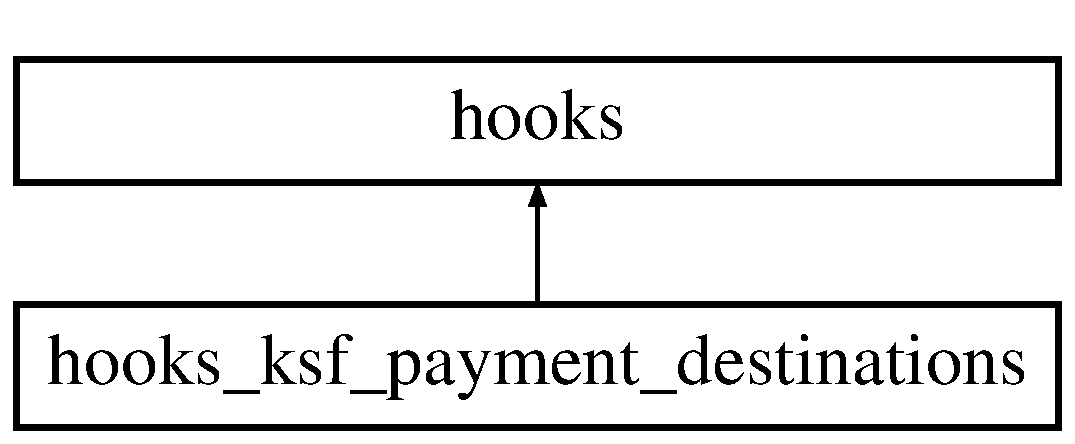
\includegraphics[height=2.000000cm]{dc/db8/classhooks__ksf__payment__destinations}
\end{center}
\end{figure}
\subsection*{Public Member Functions}
\begin{DoxyCompactItemize}
\item 
\hypertarget{classhooks__ksf__payment__destinations_a6a07b236de0c9dc8ed26c89fa490fb22}{}\label{classhooks__ksf__payment__destinations_a6a07b236de0c9dc8ed26c89fa490fb22} 
{\bfseries install\+\_\+options} (\$app)
\item 
\hypertarget{classhooks__ksf__payment__destinations_a68fb815cf25f7c3ea22cef7e04ff3e97}{}\label{classhooks__ksf__payment__destinations_a68fb815cf25f7c3ea22cef7e04ff3e97} 
{\bfseries install\+\_\+access} ()
\item 
\hypertarget{classhooks__ksf__payment__destinations_ae23102a8b3dfe29e9c8c756b9cb6bed5}{}\label{classhooks__ksf__payment__destinations_ae23102a8b3dfe29e9c8c756b9cb6bed5} 
{\bfseries db\+\_\+prewrite} (\&\$cart, \$trans\+\_\+type)
\end{DoxyCompactItemize}
\subsection*{Public Attributes}
\begin{DoxyCompactItemize}
\item 
\hypertarget{classhooks__ksf__payment__destinations_a41d2b1da19c968a3fa217d08466e8e57}{}\label{classhooks__ksf__payment__destinations_a41d2b1da19c968a3fa217d08466e8e57} 
{\bfseries \$module\+\_\+name} = \textquotesingle{}\hyperlink{classksf__payment__destinations}{ksf\+\_\+payment\+\_\+destinations}\textquotesingle{}
\end{DoxyCompactItemize}


The documentation for this class was generated from the following file\+:\begin{DoxyCompactItemize}
\item 
hooks.\+php\end{DoxyCompactItemize}

\hypertarget{classksf__payment__destinations}{}\section{ksf\+\_\+payment\+\_\+destinations Class Reference}
\label{classksf__payment__destinations}\index{ksf\+\_\+payment\+\_\+destinations@{ksf\+\_\+payment\+\_\+destinations}}
Inheritance diagram for ksf\+\_\+payment\+\_\+destinations\+:\begin{figure}[H]
\begin{center}
\leavevmode
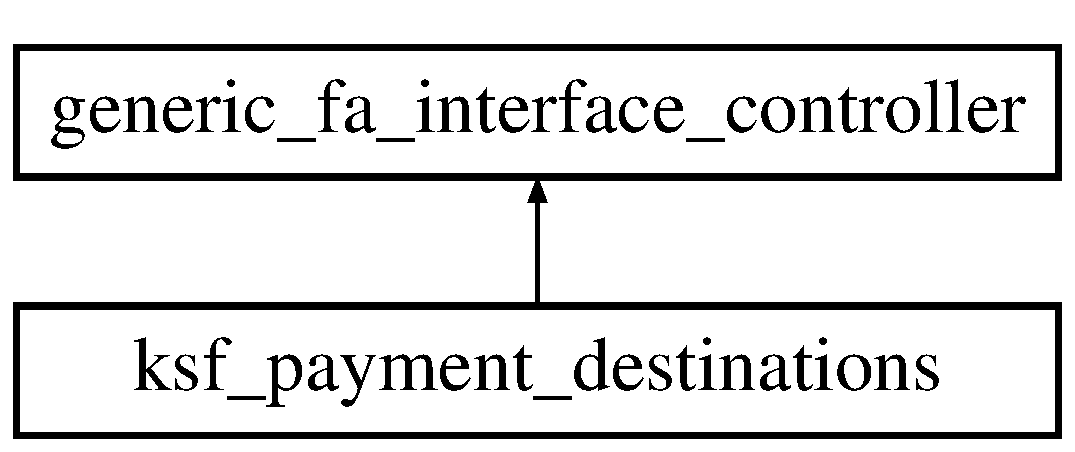
\includegraphics[height=2.000000cm]{d8/dc2/classksf__payment__destinations}
\end{center}
\end{figure}
\subsection*{Public Member Functions}
\begin{DoxyCompactItemize}
\item 
\hypertarget{classksf__payment__destinations_a3bce51ae77abebb9531554d5d6271de0}{}\label{classksf__payment__destinations_a3bce51ae77abebb9531554d5d6271de0} 
{\bfseries \+\_\+\+\_\+construct} ( \$prefs)
\item 
\hyperlink{classksf__payment__destinations_a7078c43829c1b6a6222e2930d99d0608}{handle\+\_\+edit} ()
\item 
\hyperlink{classksf__payment__destinations_a617a0cadddf6ade17f478e8476449871}{handle\+\_\+delete} ()
\item 
\hypertarget{classksf__payment__destinations_a8e3f5cc97e550f8fe1b02da3fdbf9294}{}\label{classksf__payment__destinations_a8e3f5cc97e550f8fe1b02da3fdbf9294} 
{\bfseries run} ()
\item 
\hypertarget{classksf__payment__destinations_a1e8e91ebcf8beeb203bcaf284022a586}{}\label{classksf__payment__destinations_a1e8e91ebcf8beeb203bcaf284022a586} 
{\bfseries action\+\_\+show\+\_\+form} ()
\item 
\hypertarget{classksf__payment__destinations_aa5c9b70c9fc3a4fa2909ad199303c353}{}\label{classksf__payment__destinations_aa5c9b70c9fc3a4fa2909ad199303c353} 
{\bfseries install} ()
\item 
\hyperlink{classksf__payment__destinations_af957fcc97c11896268883359ff45ddd4}{master\+\_\+form} ()
\end{DoxyCompactItemize}
\subsection*{Public Attributes}
\begin{DoxyCompactItemize}
\item 
\hypertarget{classksf__payment__destinations_a8959722e1f074ff2adf1084521a0e6af}{}\label{classksf__payment__destinations_a8959722e1f074ff2adf1084521a0e6af} 
\hyperlink{classksf__payment__destinations_a8959722e1f074ff2adf1084521a0e6af}{\$id\+\_\+ksf\+\_\+payment\+\_\+destinations}
\begin{DoxyCompactList}\small\item\em Index of table. \end{DoxyCompactList}\item 
\hypertarget{classksf__payment__destinations_ac8b962067dab478764075d7159f38e2d}{}\label{classksf__payment__destinations_ac8b962067dab478764075d7159f38e2d} 
{\bfseries \$table\+\_\+interface}
\end{DoxyCompactItemize}


\subsection{Detailed Description}
Redirect non cash payments to act like a cash payment if we have a direct invoice.

This class acts effectively as a controller.

Inherits\+: function \+\_\+\+\_\+construct( \$host, \$user, \$pass, \$database, \$pref\+\_\+tablename ) function eventloop( \$event, \$method ) function eventregister( \$event, \$method ) function add\+\_\+submodules() function module\+\_\+install() function install() function loadprefs() function updateprefs() function checkprefs() function call\+\_\+table( \$action, \$msg ) function action\+\_\+show\+\_\+form() function show\+\_\+config\+\_\+form() function form\+\_\+export() function related\+\_\+tabs() function show\+\_\+form() function base\+\_\+page() function display() function run() function modify\+\_\+table\+\_\+column( \$tables\+\_\+array ) / $\ast$@$\ast$ /function append\+\_\+file( \$filename ) /$\ast$@$\ast$ /function overwrite\+\_\+file( \$filename ) /$\ast$@$\ast$ /function open\+\_\+write\+\_\+file( \$filename ) function write\+\_\+line( \$fp, \$line ) function close\+\_\+file( \$fp ) function file\+\_\+finish( \$fp ) function backtrace() function write\+\_\+sku\+\_\+labels\+\_\+line( \$stock\+\_\+id, \$category, \$description, \$price ) function show\+\_\+generic\+\_\+form(\$form\+\_\+array) Provides\+: function \+\_\+\+\_\+construct( \$prefs ) function define\+\_\+table() function form\+\_\+ksf\+\_\+payment\+\_\+destinations function form\+\_\+ksf\+\_\+payment\+\_\+destinations\+\_\+completed function action\+\_\+show\+\_\+form() function install() function \hyperlink{classksf__payment__destinations_af957fcc97c11896268883359ff45ddd4}{master\+\_\+form()} 

\subsection{Member Function Documentation}
\hypertarget{classksf__payment__destinations_a617a0cadddf6ade17f478e8476449871}{}\label{classksf__payment__destinations_a617a0cadddf6ade17f478e8476449871} 
\index{ksf\+\_\+payment\+\_\+destinations@{ksf\+\_\+payment\+\_\+destinations}!handle\+\_\+delete@{handle\+\_\+delete}}
\index{handle\+\_\+delete@{handle\+\_\+delete}!ksf\+\_\+payment\+\_\+destinations@{ksf\+\_\+payment\+\_\+destinations}}
\subsubsection{\texorpdfstring{handle\+\_\+delete()}{handle\_delete()}}
{\footnotesize\ttfamily ksf\+\_\+payment\+\_\+destinations\+::handle\+\_\+delete (\begin{DoxyParamCaption}{ }\end{DoxyParamCaption})}

Handle the deleting from the cart of an item \hypertarget{classksf__payment__destinations_a7078c43829c1b6a6222e2930d99d0608}{}\label{classksf__payment__destinations_a7078c43829c1b6a6222e2930d99d0608} 
\index{ksf\+\_\+payment\+\_\+destinations@{ksf\+\_\+payment\+\_\+destinations}!handle\+\_\+edit@{handle\+\_\+edit}}
\index{handle\+\_\+edit@{handle\+\_\+edit}!ksf\+\_\+payment\+\_\+destinations@{ksf\+\_\+payment\+\_\+destinations}}
\subsubsection{\texorpdfstring{handle\+\_\+edit()}{handle\_edit()}}
{\footnotesize\ttfamily ksf\+\_\+payment\+\_\+destinations\+::handle\+\_\+edit (\begin{DoxyParamCaption}{ }\end{DoxyParamCaption})}

Handle the updating of the count of a stock\+\_\+id \hypertarget{classksf__payment__destinations_af957fcc97c11896268883359ff45ddd4}{}\label{classksf__payment__destinations_af957fcc97c11896268883359ff45ddd4} 
\index{ksf\+\_\+payment\+\_\+destinations@{ksf\+\_\+payment\+\_\+destinations}!master\+\_\+form@{master\+\_\+form}}
\index{master\+\_\+form@{master\+\_\+form}!ksf\+\_\+payment\+\_\+destinations@{ksf\+\_\+payment\+\_\+destinations}}
\subsubsection{\texorpdfstring{master\+\_\+form()}{master\_form()}}
{\footnotesize\ttfamily ksf\+\_\+payment\+\_\+destinations\+::master\+\_\+form (\begin{DoxyParamCaption}{ }\end{DoxyParamCaption})}

master\+\_\+form Display the summary of items with edit/delete

assumes entry\+\_\+array has been built (constructor) assumes table\+\_\+details has been built (constructor) assumes selected\+\_\+id has been set (constructor?) assumes iam has been set (constructor) 

The documentation for this class was generated from the following file\+:\begin{DoxyCompactItemize}
\item 
class.\+ksf\+\_\+payment\+\_\+destinations.\+php\end{DoxyCompactItemize}

\hypertarget{classksf__payment__destinations__model}{}\section{ksf\+\_\+payment\+\_\+destinations\+\_\+model Class Reference}
\label{classksf__payment__destinations__model}\index{ksf\+\_\+payment\+\_\+destinations\+\_\+model@{ksf\+\_\+payment\+\_\+destinations\+\_\+model}}
Inheritance diagram for ksf\+\_\+payment\+\_\+destinations\+\_\+model\+:\begin{figure}[H]
\begin{center}
\leavevmode
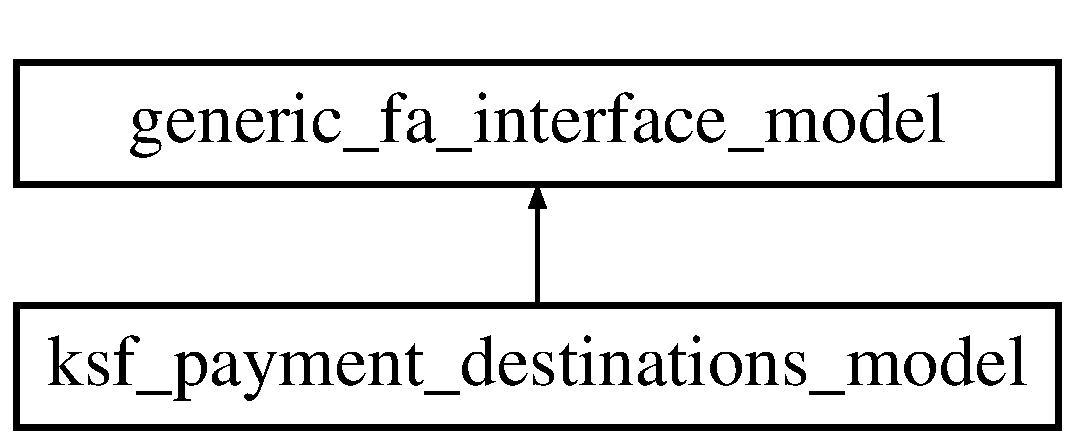
\includegraphics[height=2.000000cm]{df/df9/classksf__payment__destinations__model}
\end{center}
\end{figure}
\subsection*{Public Member Functions}
\begin{DoxyCompactItemize}
\item 
\hypertarget{classksf__payment__destinations__model_a7d2b7eaf468a2056429c887cc1c1af2c}{}\label{classksf__payment__destinations__model_a7d2b7eaf468a2056429c887cc1c1af2c} 
{\bfseries \+\_\+\+\_\+construct} ( \$prefs=ksf\+\_\+payment\+\_\+destinations\+\_\+\+P\+R\+E\+FS, \$controller)
\item 
\hypertarget{classksf__payment__destinations__model_a211128ded82e9e457860a1c025e0efa0}{}\label{classksf__payment__destinations__model_a211128ded82e9e457860a1c025e0efa0} 
{\bfseries get\+Payment\+Terms} ()
\item 
\hypertarget{classksf__payment__destinations__model_ada952f529b48c0e4060073be420098de}{}\label{classksf__payment__destinations__model_ada952f529b48c0e4060073be420098de} 
{\bfseries get\+Bank\+Account\+From\+Term} ()
\item 
\hypertarget{classksf__payment__destinations__model_a46e00553b2989537613cc99d3c9913d5}{}\label{classksf__payment__destinations__model_a46e00553b2989537613cc99d3c9913d5} 
{\bfseries define\+\_\+table} ()
\item 
\hypertarget{classksf__payment__destinations__model_a6de8af4e189cb93307bce8d6955a8b4d}{}\label{classksf__payment__destinations__model_a6de8af4e189cb93307bce8d6955a8b4d} 
{\bfseries insert\+\_\+data} ( \$arr)
\end{DoxyCompactItemize}
\subsection*{Public Attributes}
\begin{DoxyCompactItemize}
\item 
\hypertarget{classksf__payment__destinations__model_a1d84e5bee08d75539901b64c2a91ef33}{}\label{classksf__payment__destinations__model_a1d84e5bee08d75539901b64c2a91ef33} 
\hyperlink{classksf__payment__destinations__model_a1d84e5bee08d75539901b64c2a91ef33}{\$id\+\_\+ksf\+\_\+payment\+\_\+destinations}
\begin{DoxyCompactList}\small\item\em Index of table. \end{DoxyCompactList}\end{DoxyCompactItemize}
\subsection*{Protected Attributes}
\begin{DoxyCompactItemize}
\item 
\hypertarget{classksf__payment__destinations__model_ae9dd219bca42c65addf8f9eccf7269c1}{}\label{classksf__payment__destinations__model_ae9dd219bca42c65addf8f9eccf7269c1} 
\hyperlink{classksf__payment__destinations__model_ae9dd219bca42c65addf8f9eccf7269c1}{\$payment\+\_\+term}
\begin{DoxyCompactList}\small\item\em int payment type \end{DoxyCompactList}\item 
\hypertarget{classksf__payment__destinations__model_ac310931c57a514ef142670c439e1bda3}{}\label{classksf__payment__destinations__model_ac310931c57a514ef142670c439e1bda3} 
{\bfseries \$payment\+\_\+term\+\_\+name}
\item 
\hypertarget{classksf__payment__destinations__model_ade020a8ffe44944d26991547fc546d2a}{}\label{classksf__payment__destinations__model_ade020a8ffe44944d26991547fc546d2a} 
\hyperlink{classksf__payment__destinations__model_ade020a8ffe44944d26991547fc546d2a}{\$bank\+\_\+account}
\begin{DoxyCompactList}\small\item\em int GL number \end{DoxyCompactList}\item 
\hypertarget{classksf__payment__destinations__model_a43c542537d304e0ae3d37b11102b333d}{}\label{classksf__payment__destinations__model_a43c542537d304e0ae3d37b11102b333d} 
{\bfseries \$bank\+\_\+account\+\_\+name}
\end{DoxyCompactItemize}


\subsection{Detailed Description}
Inherits\+: function \+\_\+\+\_\+construct( \$host, \$user, \$pass, \$database, \$pref\+\_\+tablename ) function eventloop( \$event, \$method ) function eventregister( \$event, \$method ) function add\+\_\+submodules() function module\+\_\+install() function install() function loadprefs() function updateprefs() function checkprefs() function call\+\_\+table( \$action, \$msg ) function action\+\_\+show\+\_\+form() function show\+\_\+config\+\_\+form() function form\+\_\+export() function related\+\_\+tabs() function show\+\_\+form() function base\+\_\+page() function display() function run() function modify\+\_\+table\+\_\+column( \$tables\+\_\+array ) / $\ast$@$\ast$ /function append\+\_\+file( \$filename ) /$\ast$@$\ast$ /function overwrite\+\_\+file( \$filename ) /$\ast$@$\ast$ /function open\+\_\+write\+\_\+file( \$filename ) function write\+\_\+line( \$fp, \$line ) function close\+\_\+file( \$fp ) function file\+\_\+finish( \$fp ) function backtrace() function write\+\_\+sku\+\_\+labels\+\_\+line( \$stock\+\_\+id, \$category, \$description, \$price ) function show\+\_\+generic\+\_\+form(\$form\+\_\+array) function get( \$field ) function set( \$field, \$value = null, \$enforce = false ) function select\+\_\+row() function install() function insert\+\_\+data( \$data\+\_\+arr )

Provides\+: function \+\_\+\+\_\+construct( \$prefs = ksf\+\_\+payment\+\_\+destinations\+\_\+\+P\+R\+E\+FS, \$controller ) function get\+Payment\+Terms() function get\+Bank\+Account\+From\+Term() function define\+\_\+table() 

The documentation for this class was generated from the following file\+:\begin{DoxyCompactItemize}
\item 
class.\+ksf\+\_\+payment\+\_\+destinations\+\_\+model.\+php\end{DoxyCompactItemize}

\hypertarget{classksf__payment__destinations__view}{}\section{ksf\+\_\+payment\+\_\+destinations\+\_\+view Class Reference}
\label{classksf__payment__destinations__view}\index{ksf\+\_\+payment\+\_\+destinations\+\_\+view@{ksf\+\_\+payment\+\_\+destinations\+\_\+view}}
Inheritance diagram for ksf\+\_\+payment\+\_\+destinations\+\_\+view\+:\begin{figure}[H]
\begin{center}
\leavevmode
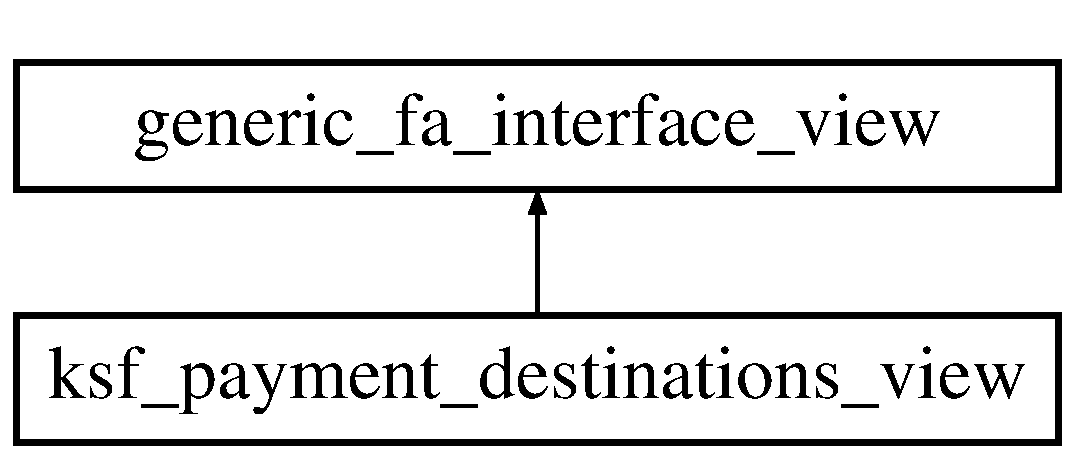
\includegraphics[height=2.000000cm]{d2/d0a/classksf__payment__destinations__view}
\end{center}
\end{figure}
\subsection*{Public Member Functions}
\begin{DoxyCompactItemize}
\item 
\hypertarget{classksf__payment__destinations__view_aede5c60959361e7283ecd91a2da3aa34}{}\label{classksf__payment__destinations__view_aede5c60959361e7283ecd91a2da3aa34} 
{\bfseries \+\_\+\+\_\+construct} ( \$prefs, \$controller)
\item 
\hypertarget{classksf__payment__destinations__view_a2128245ae36ec5b8c8ebd5650d69c24d}{}\label{classksf__payment__destinations__view_a2128245ae36ec5b8c8ebd5650d69c24d} 
{\bfseries usage\+\_\+form} ()
\item 
\hyperlink{classksf__payment__destinations__view_a9e5a6ab82c58d8f3943888a4755d6ac9}{combo\+Bank\+Account\+List} ()
\item 
\hypertarget{classksf__payment__destinations__view_a5b2f374c808923fd74fd12f84f387664}{}\label{classksf__payment__destinations__view_a5b2f374c808923fd74fd12f84f387664} 
{\bfseries combo\+Payment\+List} ()
\item 
\hypertarget{classksf__payment__destinations__view_ac6b800228e1d26f56009b98fe0e1fc73}{}\label{classksf__payment__destinations__view_ac6b800228e1d26f56009b98fe0e1fc73} 
{\bfseries form\+\_\+ksf\+\_\+payment\+\_\+destinations\+\_\+completed} ()
\item 
\hyperlink{classksf__payment__destinations__view_a5b78ad01dfa787f4445ec711ce929982}{line\+\_\+start\+\_\+focus} ()
\item 
\hypertarget{classksf__payment__destinations__view_a78ebed79bd1632f1cac1aa90b75bef70}{}\label{classksf__payment__destinations__view_a78ebed79bd1632f1cac1aa90b75bef70} 
{\bfseries form\+\_\+header} ()
\item 
\hypertarget{classksf__payment__destinations__view_ac6c5ef63c799f803fe0449136fa38b9a}{}\label{classksf__payment__destinations__view_ac6c5ef63c799f803fe0449136fa38b9a} 
{\bfseries form\+\_\+item\+\_\+rows} ()
\item 
\hypertarget{classksf__payment__destinations__view_aa5109fc69be72be0b97de639496024e9}{}\label{classksf__payment__destinations__view_aa5109fc69be72be0b97de639496024e9} 
{\bfseries form\+\_\+add} ( \$action, \$msg)
\item 
\hypertarget{classksf__payment__destinations__view_a22bdc4f15029d30d8f04c304fc82d549}{}\label{classksf__payment__destinations__view_a22bdc4f15029d30d8f04c304fc82d549} 
{\bfseries edit\+\_\+item\+\_\+form} ()
\item 
\hypertarget{classksf__payment__destinations__view_a2eb480d413a1fc6b8d696b9d85173813}{}\label{classksf__payment__destinations__view_a2eb480d413a1fc6b8d696b9d85173813} 
{\bfseries item\+\_\+form} ()
\item 
\hyperlink{classksf__payment__destinations__view_a803d4b744228624d16222728b9062f74}{master\+\_\+form} ()
\end{DoxyCompactItemize}
\subsection*{Public Attributes}
\begin{DoxyCompactItemize}
\item 
\hypertarget{classksf__payment__destinations__view_a94f35a0a472729499647d7860c9d9798}{}\label{classksf__payment__destinations__view_a94f35a0a472729499647d7860c9d9798} 
\hyperlink{classksf__payment__destinations__view_a94f35a0a472729499647d7860c9d9798}{\$id\+\_\+ksf\+\_\+payment\+\_\+destinations}
\begin{DoxyCompactList}\small\item\em Index of table. \end{DoxyCompactList}\end{DoxyCompactItemize}


\subsection{Detailed Description}
Inherits\+: function \+\_\+\+\_\+construct( \$host, \$user, \$pass, \$database, \$pref\+\_\+tablename ) function eventloop( \$event, \$method ) function eventregister( \$event, \$method ) function add\+\_\+submodules() function module\+\_\+install() function install() function loadprefs() function updateprefs() function checkprefs() function call\+\_\+table( \$action, \$msg ) function action\+\_\+show\+\_\+form() function show\+\_\+config\+\_\+form() function form\+\_\+export() function related\+\_\+tabs() function show\+\_\+form() function base\+\_\+page() function display() function run() function modify\+\_\+table\+\_\+column( \$tables\+\_\+array ) / $\ast$@$\ast$ /function append\+\_\+file( \$filename ) /$\ast$@$\ast$ /function overwrite\+\_\+file( \$filename ) /$\ast$@$\ast$ /function open\+\_\+write\+\_\+file( \$filename ) function write\+\_\+line( \$fp, \$line ) function close\+\_\+file( \$fp ) function file\+\_\+finish( \$fp ) function backtrace() function write\+\_\+sku\+\_\+labels\+\_\+line( \$stock\+\_\+id, \$category, \$description, \$price ) function show\+\_\+generic\+\_\+form(\$form\+\_\+array) Provides\+: function \+\_\+\+\_\+construct( \$prefs ) function define\+\_\+table() function form\+\_\+\+Payment Type to Bank Account function form\+\_\+\+Payment Type to Bank Account\+\_\+completed function action\+\_\+show\+\_\+form()

function \hyperlink{classksf__payment__destinations__view_a803d4b744228624d16222728b9062f74}{master\+\_\+form()} 

\subsection{Member Function Documentation}
\hypertarget{classksf__payment__destinations__view_a9e5a6ab82c58d8f3943888a4755d6ac9}{}\label{classksf__payment__destinations__view_a9e5a6ab82c58d8f3943888a4755d6ac9} 
\index{ksf\+\_\+payment\+\_\+destinations\+\_\+view@{ksf\+\_\+payment\+\_\+destinations\+\_\+view}!combo\+Bank\+Account\+List@{combo\+Bank\+Account\+List}}
\index{combo\+Bank\+Account\+List@{combo\+Bank\+Account\+List}!ksf\+\_\+payment\+\_\+destinations\+\_\+view@{ksf\+\_\+payment\+\_\+destinations\+\_\+view}}
\subsubsection{\texorpdfstring{combo\+Bank\+Account\+List()}{comboBankAccountList()}}
{\footnotesize\ttfamily ksf\+\_\+payment\+\_\+destinations\+\_\+view\+::combo\+Bank\+Account\+List (\begin{DoxyParamCaption}{ }\end{DoxyParamCaption})}

Using FA routine display a combo box of bank accounts \hypertarget{classksf__payment__destinations__view_a5b78ad01dfa787f4445ec711ce929982}{}\label{classksf__payment__destinations__view_a5b78ad01dfa787f4445ec711ce929982} 
\index{ksf\+\_\+payment\+\_\+destinations\+\_\+view@{ksf\+\_\+payment\+\_\+destinations\+\_\+view}!line\+\_\+start\+\_\+focus@{line\+\_\+start\+\_\+focus}}
\index{line\+\_\+start\+\_\+focus@{line\+\_\+start\+\_\+focus}!ksf\+\_\+payment\+\_\+destinations\+\_\+view@{ksf\+\_\+payment\+\_\+destinations\+\_\+view}}
\subsubsection{\texorpdfstring{line\+\_\+start\+\_\+focus()}{line\_start\_focus()}}
{\footnotesize\ttfamily ksf\+\_\+payment\+\_\+destinations\+\_\+view\+::line\+\_\+start\+\_\+focus (\begin{DoxyParamCaption}{ }\end{DoxyParamCaption})}

Set the focus on the cart\textquotesingle{}s displayed table

\begin{DoxyReturn}{Returns}
N\+O\+NE 
\end{DoxyReturn}
\hypertarget{classksf__payment__destinations__view_a803d4b744228624d16222728b9062f74}{}\label{classksf__payment__destinations__view_a803d4b744228624d16222728b9062f74} 
\index{ksf\+\_\+payment\+\_\+destinations\+\_\+view@{ksf\+\_\+payment\+\_\+destinations\+\_\+view}!master\+\_\+form@{master\+\_\+form}}
\index{master\+\_\+form@{master\+\_\+form}!ksf\+\_\+payment\+\_\+destinations\+\_\+view@{ksf\+\_\+payment\+\_\+destinations\+\_\+view}}
\subsubsection{\texorpdfstring{master\+\_\+form()}{master\_form()}}
{\footnotesize\ttfamily ksf\+\_\+payment\+\_\+destinations\+\_\+view\+::master\+\_\+form (\begin{DoxyParamCaption}{ }\end{DoxyParamCaption})}

master\+\_\+form Display the summary of items with edit/delete

assumes entry\+\_\+array has been built (constructor) assumes table\+\_\+details has been built (constructor) assumes selected\+\_\+id has been set (constructor?) assumes iam has been set (constructor) 

The documentation for this class was generated from the following file\+:\begin{DoxyCompactItemize}
\item 
class.\+ksf\+\_\+payment\+\_\+destinations\+\_\+view.\+php\end{DoxyCompactItemize}

%--- End generated contents ---

% Index
\backmatter
\newpage
\phantomsection
\clearemptydoublepage
\addcontentsline{toc}{chapter}{Index}
\printindex

\end{document}
